% The four end conditions of the Euler--Bernoulli beam.
% In each panel: the left end of the beam at rest (dashed) and deflected (blue).
% Shared by the lecture notes and the slides.
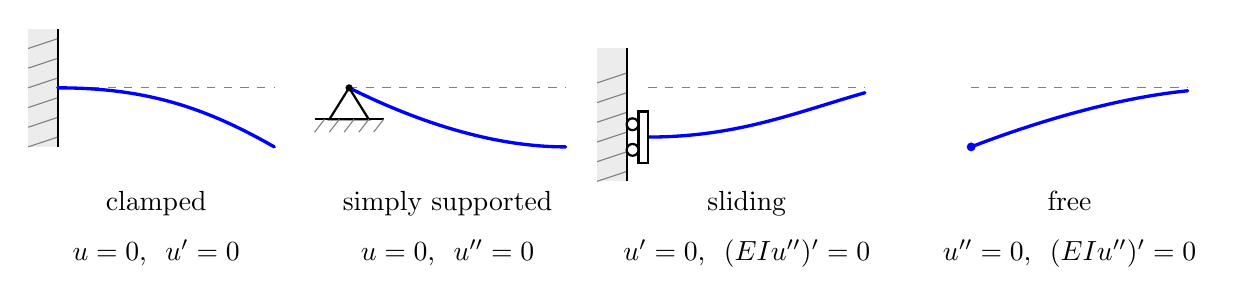
\begin{tikzpicture}[x=1.25cm,y=1.25cm]
    \tikzset{
        rest/.style={gray,dashed},
        beam/.style={very thick,blue,line cap=round},
        support/.style={thick},
        hatch/.style={gray},
    }
    % clamped: the wall fixes the position and the slope
    \begin{scope}
        \fill[gray!15] (-.3,-.6) rectangle (0,.6);
        \foreach \y in {-.5,-.3,...,.55} \draw[hatch] (0,\y) -- ++(-.3,-.1);
        \draw[support] (0,-.6) -- (0,.6);
        \draw[rest] (0,0) -- (2.2,0);
        \draw[beam] (0,0) .. controls (.9,0) and (1.5,-.2) .. (2.2,-.6);
        \node[anchor=base] at (1,-1.25) {clamped};
        \node[anchor=base] at (1,-1.75) {$u = 0$, \ $u' = 0$};
    \end{scope}
    % simply supported: the hinge fixes the position, the end rotates
    \begin{scope}[xshift=3.7cm]
        \draw[rest] (0,0) -- (2.2,0);
        \draw[beam] (0,0) .. controls (.6,-.3) and (1.4,-.6) .. (2.2,-.6);
        \draw[support,fill=white] (0,0) -- (-.2,-.32) -- (.2,-.32) -- cycle;
        \draw[support] (-.35,-.32) -- (.35,-.32);
        \foreach \x in {-.25,-.1,...,.36} \draw[hatch] (\x,-.32) -- ++(-.1,-.13);
        \fill (0,0) circle (1.3pt);
        \node[anchor=base] at (1,-1.25) {simply supported};
        \node[anchor=base] at (1,-1.75) {$u = 0$, \ $u'' = 0$};
    \end{scope}
    % sliding: the end moves along the wall, the slope is fixed
    \begin{scope}[xshift=7.5cm]
        \fill[gray!15] (-.52,-.95) rectangle (-.22,.4);
        \foreach \y in {-.85,-.65,...,.35} \draw[hatch] (-.22,\y) -- ++(-.3,-.1);
        \draw[support] (-.22,-.95) -- (-.22,.4);
        \draw[rest] (0,0) -- (2.2,0);
        \draw[beam] (0,-.5) .. controls (.9,-.5) and (1.5,-.25) .. (2.2,-.05);
        \draw[support,fill=white] (-.1,-.76) rectangle (0,-.24);
        \draw[support,fill=white] (-.16,-.63) circle (.06);
        \draw[support,fill=white] (-.16,-.37) circle (.06);
        \node[anchor=base] at (1,-1.25) {sliding};
        \node[anchor=base] at (1,-1.75) {$u' = 0$, \ $(EI u'')' = 0$};
    \end{scope}
    % free: no force and no moment
    \begin{scope}[xshift=11.6cm]
        \draw[rest] (0,0) -- (2.2,0);
        \draw[beam] (0,-.6) .. controls (.7,-.33) and (1.5,-.1) .. (2.2,-.03);
        \fill[blue] (0,-.6) circle (1.6pt);
        \node[anchor=base] at (1,-1.25) {free};
        \node[anchor=base] at (1,-1.75) {$u'' = 0$, \ $(EI u'')' = 0$};
    \end{scope}
\end{tikzpicture}
